\documentclass[10pt,twocolumn]{article}
\usepackage[margin=0.75in]{geometry}
\usepackage{graphicx,booktabs,amsmath,hyperref,xcolor,multirow}
\newcommand{\todo}[1]{\textcolor{red}{[#1]}}

\title{Where Does a Vision Transformer Need Adaptation Capacity under Domain Shift?\\
\large A Study of LoRA Placement, Layer-wise Rank, and 4-bit (QLoRA) Compression on PACS and Office-Home}
\author{\todo{Author name} \\ \todo{Affiliation}}
\date{}

\begin{document}
\maketitle

\begin{abstract}
Image classifiers lose accuracy when the visual style of the test images differs from the training images
(domain shift). Parameter-efficient fine-tuning (PEFT) adapts a frozen pretrained model with few trainable
parameters, and LoRA is the most widely used PEFT method, but it is usually applied with one fixed rank in every
layer, a recipe inherited from language models. We ask where inside a Vision Transformer the adaptation capacity
is actually useful under domain shift. With a frozen ViT-B/16 and the leave-one-domain-out protocol on PACS and
Office-Home, we compare, at matched parameter budgets, LoRA in early, middle and late blocks; uniform versus
layer-wise rank allocations; attention versus MLP projections; and a 4-bit NF4 (QLoRA) backbone, against linear
probing and BitFit. Spreading a small rank over all blocks was best: at the same budget, adapters only in the late blocks lost 6.7 points on PACS (and were worst on Sketch), rank 1 was within 0.7 points of rank 4 while rank 16 was lower, and depth-wise rank profiles did not beat uniform rank. MLP adapters beat attention adapters at a matched budget on both datasets (+1.0 and +1.1 points). A 4-bit backbone cost at most 0.5 points, but at ViT-B scale it raised peak training memory by about 25\%, because activations rather than weights dominate. The trends transfer to Office-Home with smaller gaps.
\end{abstract}

\section{Introduction}
Deep image classifiers are trained and tested on images that look alike. When the style changes, for example
from photographs to sketches, accuracy drops sharply even though the objects are the same. This domain shift is
the norm in practice, and retraining an entire model for each new visual domain is expensive.

Parameter-efficient fine-tuning keeps a large pretrained backbone frozen and trains a small number of new
parameters. LoRA~\cite{hu2021lora} adds a trainable low-rank update $BA$ to selected weight matrices and has
become the default PEFT method. QLoRA~\cite{dettmers2023qlora} additionally stores the frozen weights in 4-bit
NormalFloat (NF4) precision to reduce memory. Both were developed for large language models, where LoRA is
typically placed on the attention projections of every layer with one shared rank.

For Vision Transformers (ViTs)~\cite{dosovitskiy2021vit} under domain shift, it is not well understood whether
this default is a good use of a fixed parameter budget. Early ViT blocks encode low-level appearance (texture,
color, stroke), which is exactly what changes between domains, while late blocks encode more semantic
features. This suggests that the location of the adapters, and how rank is distributed across depth, may matter
more than the total number of parameters.

We run a controlled study that holds the backbone, data, protocol and parameter budget fixed and varies only
where the capacity goes. Our questions are:
\textbf{RQ1} With the same budget, are adapters better in early, middle, or late blocks?
\textbf{RQ2} How small can the rank be, and does a layer-wise rank allocation beat a uniform one?
\textbf{RQ3} Do attention or MLP projections benefit more from LoRA?
\textbf{RQ4} How much accuracy does a 4-bit backbone cost, and how much memory does it save?
\textbf{RQ5} Do the PACS findings transfer to Office-Home?

Our contribution is empirical: a budget-matched comparison of existing techniques with practical guidance,
rather than a new adaptation method.

\section{Related Work}
\textbf{Domain generalization.} PACS~\cite{li2017pacs} and Office-Home~\cite{venkateswara2017officehome} are
standard multi-domain benchmarks. DomainBed~\cite{gulrajani2021domainbed} showed that, under a fair protocol with
model selection on source-domain validation data, plain empirical risk minimization is a strong baseline; we
follow its leave-one-domain-out protocol and training-domain validation.

\textbf{Parameter-efficient fine-tuning.} Besides LoRA, BitFit~\cite{zaken2022bitfit} trains only bias terms,
adapter methods such as AdaptFormer~\cite{chen2022adaptformer} insert small bottleneck modules into ViTs, and
visual prompt tuning~\cite{jia2022vpt} learns extra input tokens. AdaLoRA~\cite{zhang2023adalora} learns the rank
allocation across weight matrices during training. Our study instead fixes simple, interpretable allocations
(early/middle/late, increasing/decreasing) at a matched budget, so the effect of position and depth can be read
off directly. \todo{verify all references; add 2-3 recent PEFT-for-DG papers}

\textbf{Quantized fine-tuning.} QLoRA~\cite{dettmers2023qlora} fine-tunes LoRA adapters on top of a 4-bit NF4
backbone and is designed for billion-parameter language models, where frozen weights dominate memory. We measure
whether the same trade-off holds for an 86M-parameter ViT.

\section{Method}
\begin{figure*}[t]
\centering
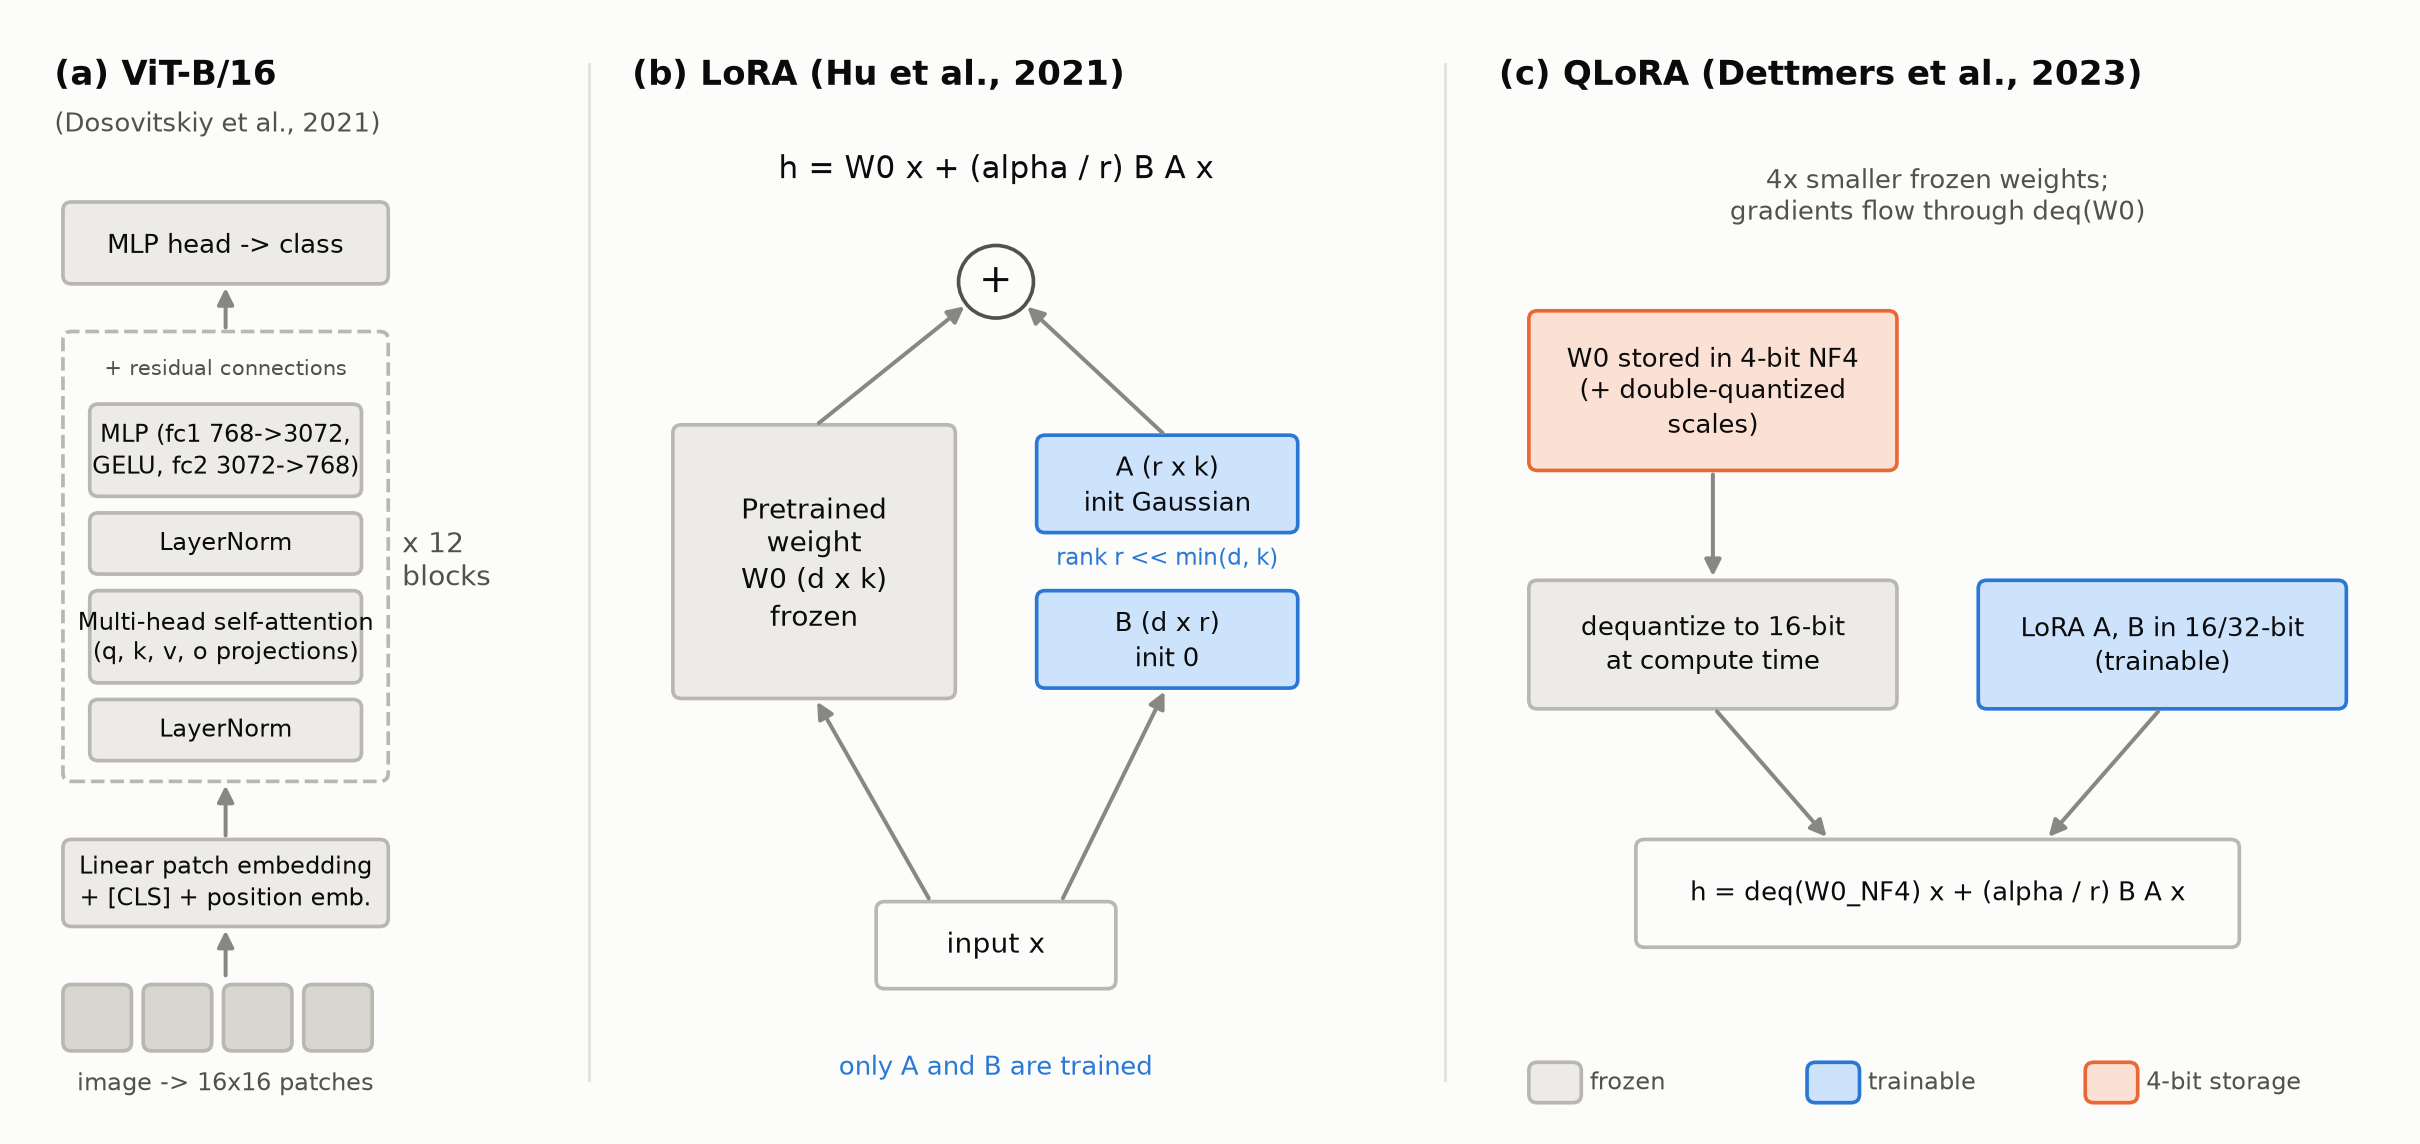
\includegraphics[width=0.85\textwidth]{../figures/fig1_base_paper_architecture.png}
\caption{Base methods. (a) ViT encoder. (b) LoRA: a frozen weight $W_0$ plus a trainable low-rank update
$\frac{\alpha}{r}BA$. (c) QLoRA: $W_0$ is stored in 4-bit NF4 and dequantized at compute time.}
\label{fig:base}
\end{figure*}

\begin{figure*}[t]
\centering
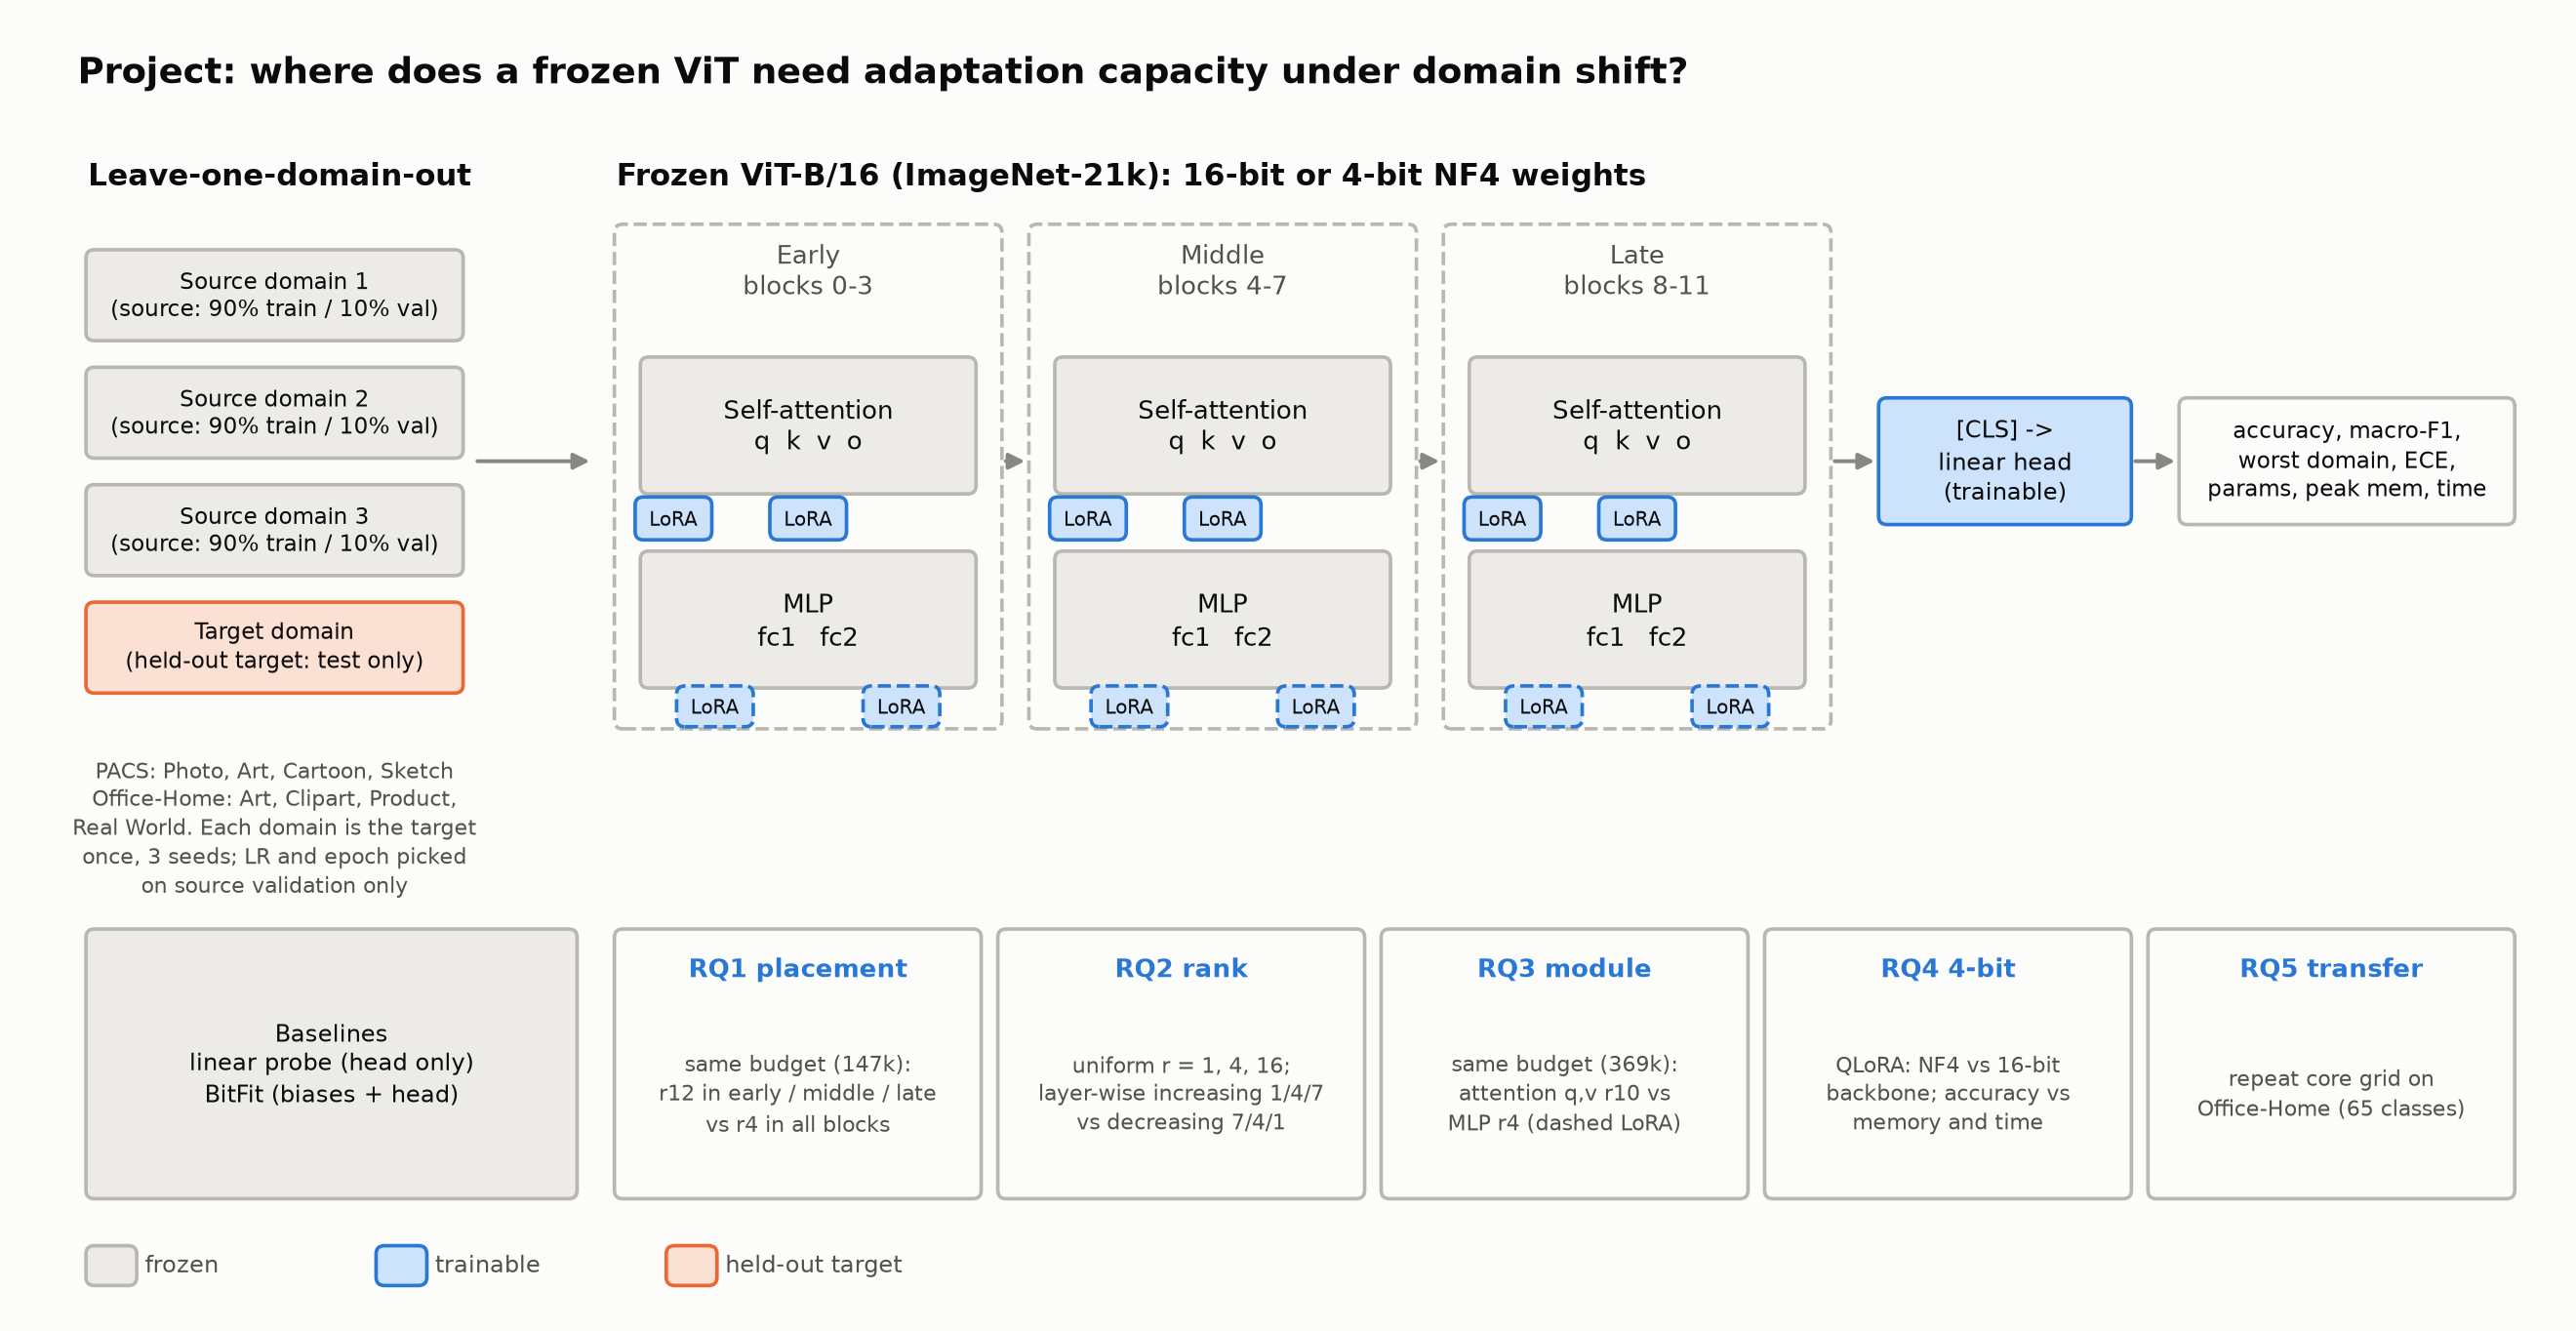
\includegraphics[width=0.95\textwidth]{../figures/fig2_project_architecture.png}
\caption{Study design. A frozen ViT-B/16 is adapted with LoRA in different groups of blocks, on attention ($q,v$)
or MLP ($fc_1, fc_2$) projections, with a 16-bit or 4-bit backbone, under leave-one-domain-out evaluation.}
\label{fig:project}
\end{figure*}

\textbf{Backbone.} ViT-B/16 pretrained on ImageNet-21k (\texttt{google/vit-base-patch16-224-in21k}), 12 blocks,
width 768, MLP width 3072. All backbone weights are frozen and kept in 16-bit precision (or 4-bit NF4 for QLoRA).
A new linear classification head on the [CLS] token is always trained.

\textbf{LoRA.} For a frozen linear map $W_0\in\mathbb{R}^{d\times k}$ we learn $h = W_0x + \frac{\alpha}{r}BAx$
with $A\in\mathbb{R}^{r\times k}$, $B\in\mathbb{R}^{d\times r}$, $B$ initialized to zero, $\alpha=2r$ and dropout
0.1 on the LoRA input. A rank-$r$ adapter on a $768{\times}768$ attention projection has $1536r$ parameters; on
$fc_1$ or $fc_2$ it has $3840r$.

\textbf{Configurations} (Table~\ref{tab:configs}). We split the 12 blocks into early (0--3), middle (4--7) and late
(8--11) thirds. \emph{Placement} (RQ1): rank 12 on $q,v$ in only one third, which equals the budget of rank 4 in all
blocks (147{,}456 adapter parameters). \emph{Rank} (RQ2): uniform $r\in\{1,4,16\}$, and layer-wise allocations
increasing (1/4/7 per third) or decreasing (7/4/1), both with the same total rank as uniform $r=4$.
\emph{Module} (RQ3): attention $q,v$ with $r=10$ versus MLP $fc_1,fc_2$ with $r=4$, both 368{,}640 parameters.
\emph{Quantization} (RQ4): uniform $r=4$ on a 4-bit NF4 backbone with double quantization (QLoRA) versus the same
adapters on the 16-bit backbone. \emph{Baselines}: linear probing (head only) and BitFit (all biases plus head).

\begin{table}[t]
\centering\small
\begin{tabular}{llr}
\toprule
Config & LoRA ranks (early/mid/late) & Adapter params \\
\midrule
Linear probe & -- & 0 \\
BitFit & biases & 102{,}912 \\
All $r$1 / $r$4 / $r$16 & $q,v$: 1/1/1, 4/4/4, 16/16/16 & 37k / 147k / 590k \\
Early / Middle / Late & $q,v$: 12/0/0, 0/12/0, 0/0/12 & 147{,}456 \\
Increasing / Decreasing & $q,v$: 1/4/7, 7/4/1 & 147{,}456 \\
Attention $r$10 & $q,v$: 10/10/10 & 368{,}640 \\
MLP $r$4 & $fc_1,fc_2$: 4/4/4 & 368{,}640 \\
QLoRA $r$4 & $q,v$: 4/4/4, NF4 backbone & 147{,}456 \\
\bottomrule
\end{tabular}
\caption{Configurations. The head adds $768C{+}C$ parameters ($C$ = number of classes) to every method.}
\label{tab:configs}
\end{table}

\section{Experimental Setup}
\textbf{Data.} PACS~\cite{li2017pacs}: 9{,}991 images, 7 classes, domains Photo, Art painting, Cartoon, Sketch.
Office-Home~\cite{venkateswara2017officehome}: 15{,}588 images, 65 classes, domains Art, Clipart, Product, Real
World. Both are loaded from the Hugging Face Hub (\texttt{flwrlabs/pacs}, \texttt{flwrlabs/office-home}).

\textbf{Protocol.} Leave-one-domain-out: three source domains are split 90/10 into train and validation (fixed split,
independent of the training seed), and the held-out target domain is used only for testing. Model selection,
both learning rate and best epoch, uses source validation accuracy only. Each configuration is run for every
target domain with 3 seeds. PACS uses 13 configurations (Table~\ref{tab:configs}); Office-Home uses a reduced set of 8 (linear probe, BitFit, LoRA $r$=4, early, late, attention $r$=10, MLP $r$=4, QLoRA $r$=4).

\textbf{Training.} AdamW, weight decay 0.01 (0 for BitFit), batch 64, 4 epochs, 5\% linear warm-up then cosine
decay, label smoothing 0.1, mixed precision. Augmentation: random resized crop (scale 0.6--1) to 224, horizontal
flip, color jitter. The learning rate per method (linear probe, BitFit, LoRA) is chosen from
$\{10^{-3}, 3{\cdot}10^{-3}, 10^{-2}\}$ on one split (target Art painting for PACS, Art for Office-Home) by source validation accuracy. Both datasets selected $10^{-2}$ for the linear probe and BitFit and $3{\cdot}10^{-3}$ for LoRA; all LoRA and QLoRA variants share the LoRA learning rate.

\textbf{Metrics.} Target accuracy and macro-F1, averaged over target domains (``avg'') and the minimum over
targets (``worst''), expected calibration error (15 bins), trainable parameters, peak GPU memory during
training (\texttt{torch.cuda.max\_memory\_allocated}), and training time.

\textbf{Hardware.} PACS runs used NVIDIA Tesla T4 GPUs (Kaggle); Office-Home runs used an AMD Radeon RX 9070
GRE (ROCm 7.2). Memory and time are only compared within one dataset, i.e.\ on the same hardware.

\section{Results}
\begin{table*}[t]
\centering\small
\begin{tabular}{lrrrrrrrrrr}
\toprule
Method & Art & Cart. & Photo & Sketch & Avg & Worst & F1 & Params & Mem & Time \\
\midrule
Linear probe & 82.4 & 67.0 & 95.4 & 33.4 & 69.5$\pm$0.8 & 33.4 & 72.3 & 0 & 0.84 & 91 \\
BitFit & 92.2 & 87.0 & 99.6 & 72.0 & \textbf{87.7$\pm$0.3} & 72.0 & 88.3 & 103k & 3.07 & 182 \\
\midrule
LoRA all, $r$=1 & 93.1 & 84.2 & 99.8 & 69.0 & 86.5$\pm$1.4 & 69.0 & 87.1 & 37k & 3.66 & 207 \\
LoRA all, $r$=4 & 94.0 & 85.3 & 99.7 & 69.8 & 87.2$\pm$0.7 & 69.8 & 87.8 & 147k & 3.65 & 202 \\
LoRA all, $r$=16 & 92.3 & 84.9 & 99.7 & 64.3 & 85.3$\pm$1.4 & 64.3 & 86.0 & 590k & 3.66 & 204 \\
\midrule
Early (0--3), $r$=12 & 89.9 & 82.3 & 99.8 & 68.4 & 85.1$\pm$0.1 & 68.4 & 85.6 & 147k & 3.21 & 185 \\
Middle (4--7), $r$=12 & 91.9 & 81.4 & 99.9 & 66.6 & 85.0$\pm$1.0 & 66.6 & 85.7 & 147k & 2.34 & 153 \\
Late (8--11), $r$=12 & 92.1 & 78.9 & 99.5 & 51.6 & 80.5$\pm$1.2 & 51.6 & 81.8 & 147k & 1.47 & 121 \\
\midrule
Increasing 1/4/7 & 94.0 & 85.2 & 99.7 & 67.0 & 86.5$\pm$1.0 & 67.0 & 87.3 & 147k & 3.64 & 206 \\
Decreasing 7/4/1 & 93.0 & 85.0 & 99.9 & 67.7 & 86.4$\pm$1.1 & 67.7 & 87.0 & 147k & 3.64 & 206 \\
\midrule
Attention $q,v$, $r$=10 & 93.3 & 85.2 & 99.4 & 67.4 & 86.4$\pm$0.5 & 67.4 & 86.9 & 369k & 3.65 & 205 \\
MLP $fc_1,fc_2$, $r$=4 & 94.2 & 86.0 & 99.7 & 69.6 & 87.4$\pm$1.6 & 69.6 & 88.3 & 369k & 4.81 & 245 \\
\midrule
QLoRA $r$=4 (NF4) & 93.3 & 85.5 & 99.7 & 69.7 & 87.1$\pm$0.4 & 69.7 & 87.6 & 147k & 4.55 & 249 \\
\bottomrule
\end{tabular}
\caption{PACS, ViT-B/16, Tesla T4. Target-domain accuracy (\%) per held-out domain, mean over 3 seeds; Avg $\pm$ sd over seeds of the domain-averaged accuracy; Worst = lowest held-out domain; F1 = macro-F1 averaged over domains; Params = trainable parameters excluding the head; Mem = peak training memory (GB); Time = training seconds per run.}
\label{tab:pacs}
\end{table*}
\begin{table*}[t]
\centering\small
\begin{tabular}{lrrrrrrrrrr}
\toprule
Method & Art & Clip. & Prod. & Real & Avg & Worst & F1 & Params & Mem & Time \\
\midrule
Linear probe & 79.2 & 59.0 & 88.4 & 89.6 & 79.0$\pm$0.1 & 59.0 & 78.0 & 0 & 1.03 & 91 \\
BitFit & 80.4 & 64.2 & 88.4 & 89.1 & 80.5$\pm$0.2 & 64.2 & 79.4 & 103k & 3.26 & 150 \\
LoRA all, $r$=4 & 82.6 & 63.2 & 89.1 & 90.7 & 81.4$\pm$0.2 & 63.2 & 80.4 & 147k & 3.81 & 170 \\
\midrule
Early (0--3), $r$=12 & 81.5 & 63.5 & 89.0 & 90.5 & 81.1$\pm$0.3 & 63.5 & 80.0 & 147k & 3.37 & 152 \\
Late (8--11), $r$=12 & 81.8 & 61.0 & 89.2 & 90.3 & 80.6$\pm$0.2 & 61.0 & 79.6 & 147k & 1.63 & 115 \\
\midrule
Attention $q,v$, $r$=10 & 81.3 & 62.9 & 88.5 & 90.3 & 80.7$\pm$0.2 & 62.9 & 79.8 & 369k & 3.78 & 169 \\
MLP $fc_1,fc_2$, $r$=4 & 82.6 & 65.0 & 89.0 & 90.6 & \textbf{81.8$\pm$0.1} & 65.0 & 80.7 & 369k & 4.93 & 216 \\
\midrule
QLoRA $r$=4 (NF4) & 82.1 & 62.2 & 88.9 & 90.5 & 80.9$\pm$0.1 & 62.2 & 80.0 & 147k & 4.69 & 223 \\
\bottomrule
\end{tabular}
\caption{Office-Home, ViT-B/16, RX 9070 GRE. Target-domain accuracy (\%) per held-out domain, mean over 3 seeds; Avg $\pm$ sd over seeds of the domain-averaged accuracy; Worst = lowest held-out domain; F1 = macro-F1 averaged over domains; Params = trainable parameters excluding the head; Mem = peak training memory (GB); Time = training seconds per run.}
\label{tab:oh}
\end{table*}
\begin{table}[t]
\centering\small
\begin{tabular}{lrrrr}
\toprule
Comparison (A vs B) & \multicolumn{2}{c}{PACS} & \multicolumn{2}{c}{Office-Home} \\
 & $\Delta$ & $p$ & $\Delta$ & $p$ \\
\midrule
Early (0--3), $r$=12 vs LoRA all, $r$=4 & -2.1 & 0.003 & -0.2 & 0.223 \\
Middle (4--7), $r$=12 vs LoRA all, $r$=4 & -2.2 & 0.015 & -- & -- \\
Late (8--11), $r$=12 vs LoRA all, $r$=4 & -6.7 & 0.010 & -0.8 & 0.025 \\
Early (0--3), $r$=12 vs Late (8--11), $r$=12 & +4.6 & 0.069 & +0.6 & 0.198 \\
Middle (4--7), $r$=12 vs Late (8--11), $r$=12 & +4.4 & 0.055 & -- & -- \\
Early (0--3), $r$=12 vs Middle (4--7), $r$=12 & +0.1 & 0.809 & -- & -- \\
LoRA all, $r$=1 vs LoRA all, $r$=4 & -0.7 & 0.305 & -- & -- \\
LoRA all, $r$=16 vs LoRA all, $r$=4 & -1.9 & 0.150 & -- & -- \\
Increasing 1/4/7 vs LoRA all, $r$=4 & -0.7 & 0.298 & -- & -- \\
Decreasing 7/4/1 vs LoRA all, $r$=4 & -0.8 & 0.167 & -- & -- \\
Increasing 1/4/7 vs Decreasing 7/4/1 & +0.1 & 0.934 & -- & -- \\
MLP $fc_1,fc_2$, $r$=4 vs Attention $q,v$, $r$=10 & +1.0 & 0.221 & +1.1 & 0.004 \\
QLoRA $r$=4 (NF4) vs LoRA all, $r$=4 & -0.1 & 0.781 & -0.5 & 0.004 \\
LoRA all, $r$=4 vs BitFit & -0.5 & 0.351 & +0.8 & 0.048 \\
LoRA all, $r$=4 vs Linear probe & +17.7 & 0.001 & +2.3 & 0.000 \\
BitFit vs Linear probe & +18.2 & 0.001 & +1.5 & 0.060 \\
\bottomrule
\end{tabular}
\caption{Paired comparisons: mean accuracy difference A$-$B in points over the 12 matched (target domain, seed) runs, and two-sided paired $t$-test $p$-value.}
\label{tab:tests}
\end{table}


\begin{figure}[t]
\centering
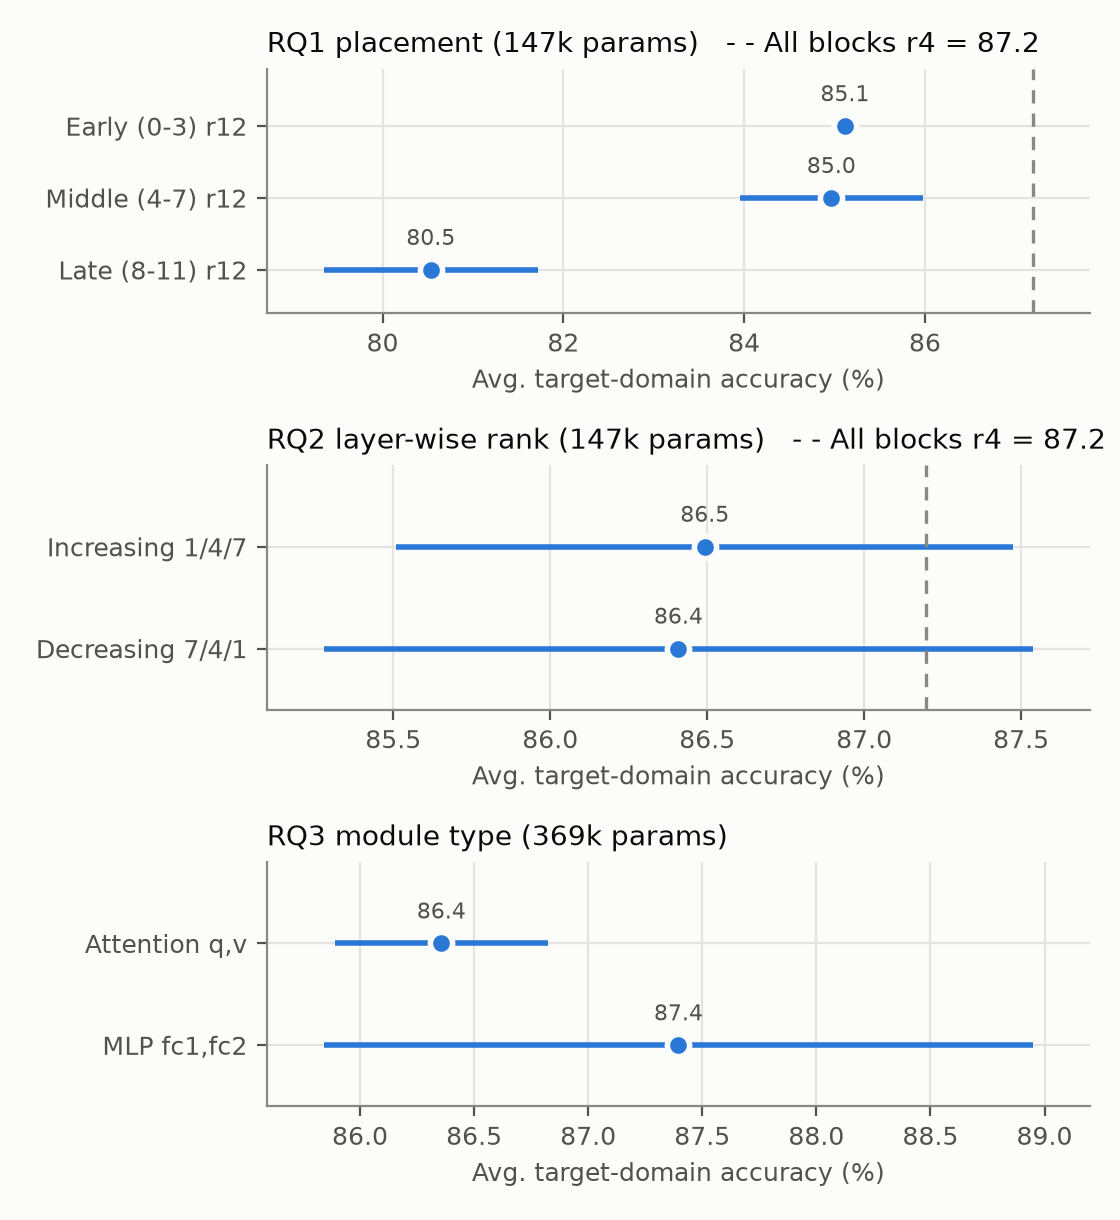
\includegraphics[width=\columnwidth]{../figures/pacs_vit_b_e4_placement_rank_module.png}
\caption{PACS, budget-matched comparisons (mean $\pm$ sd over seeds). Dashed line: LoRA $r$=4 in all blocks, same
budget as the placement and layer-wise variants.}
\label{fig:pacs-panels}
\end{figure}

\begin{figure}[t]
\centering
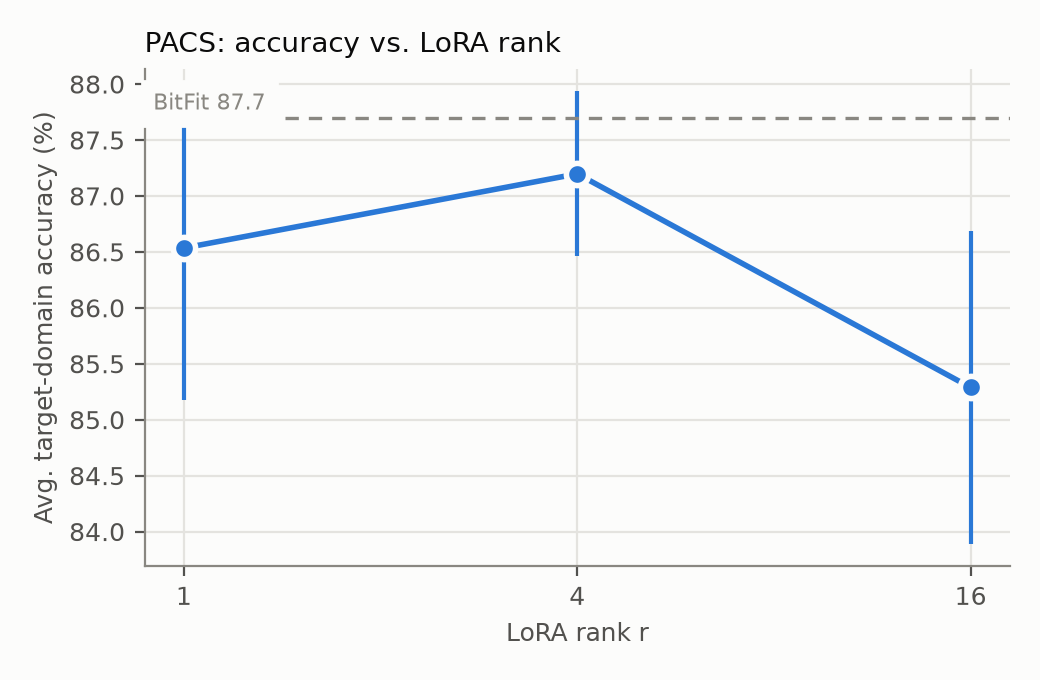
\includegraphics[width=\columnwidth]{../figures/pacs_vit_b_e4_rank.png}
\caption{PACS, accuracy versus uniform LoRA rank (all blocks, $q,v$). Dashed: BitFit. The linear probe (69.5\%) is
off the scale.}
\label{fig:rank}
\end{figure}

\begin{figure*}[t]
\centering
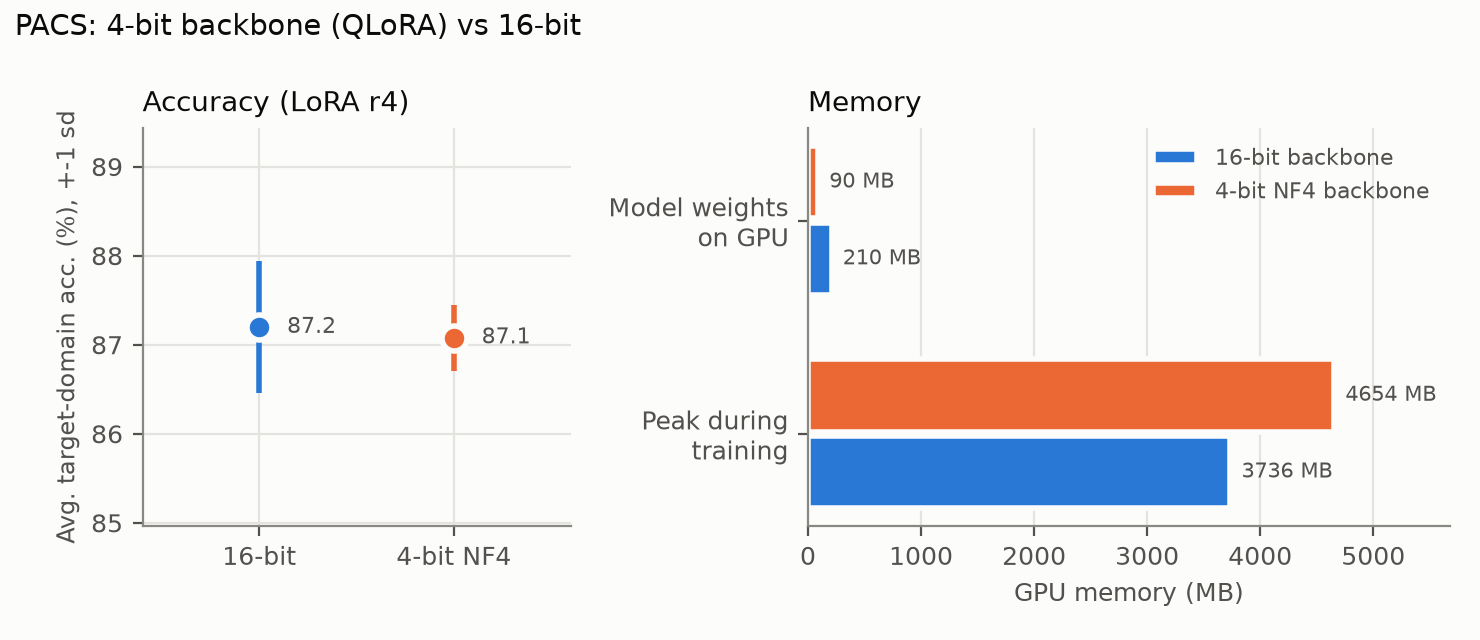
\includegraphics[width=0.49\textwidth]{../figures/pacs_vit_b_e4_qlora.png}\hfill
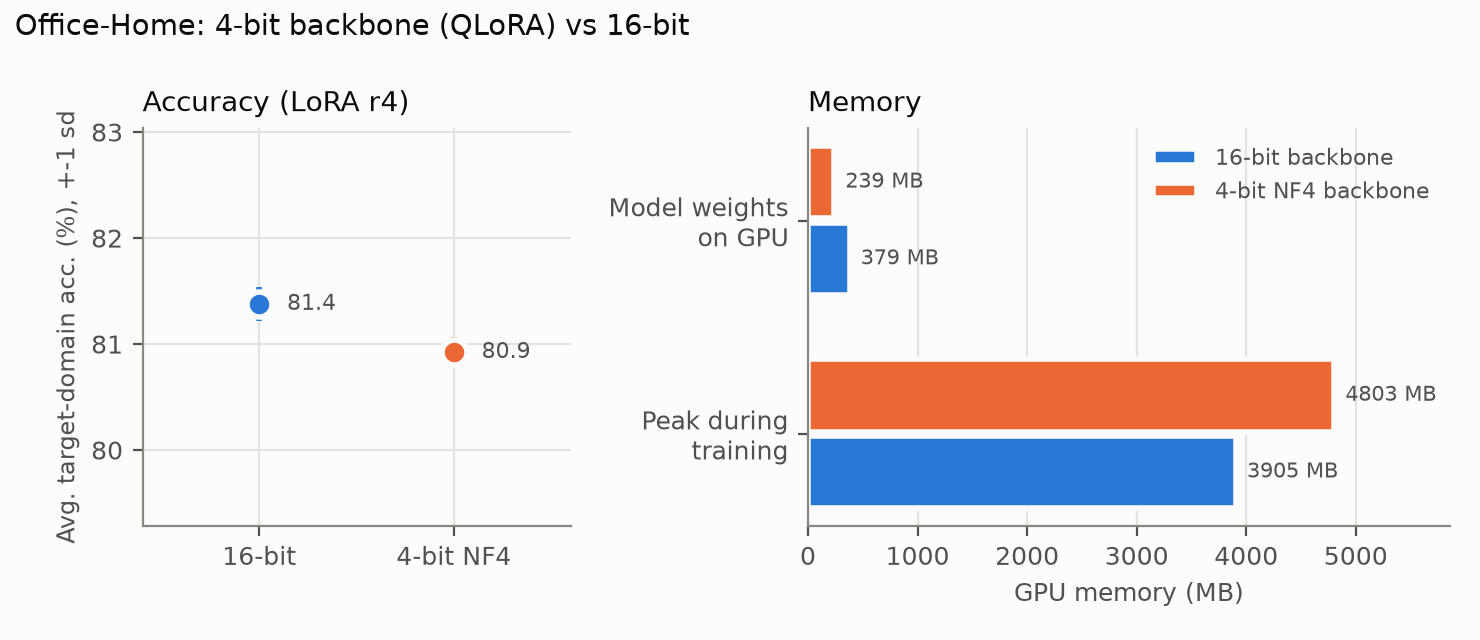
\includegraphics[width=0.49\textwidth]{../figures/officehome_vit_b_e4_qlora.png}
\caption{4-bit NF4 backbone (QLoRA) versus the same LoRA $r$=4 adapters on a 16-bit backbone. Left: PACS (Tesla T4).
Right: Office-Home (RX 9070 GRE). The 4-bit backbone shrinks the stored weights but raises peak training memory.}
\label{fig:qlora}
\end{figure*}

Tables~\ref{tab:pacs} and~\ref{tab:oh} give the full results and Table~\ref{tab:tests} the paired tests. Any
trainable adaptation beats the linear probe, by a wide margin on PACS (+17.7 points for LoRA $r$=4, $p<0.001$) and
a smaller one on Office-Home (+2.3), and the hardest target is always the most stylized domain (Sketch, Clipart).

\subsection{RQ1: Placement}
At a fixed budget of 147k parameters, concentrating rank in one third of the network is worse than spreading rank 4
over all 12 blocks: on PACS by 2.1 (early, $p=0.003$), 2.2 (middle, $p=0.015$) and 6.7 points (late, $p=0.010$;
lower in all 12 paired runs). Late-only adaptation is clearly the worst placement: on the Sketch target it reaches
51.6\% versus 68.4\% for early-only and 69.8\% for all blocks. Early and middle placement are indistinguishable
($+0.15$, $p=0.81$). Office-Home shows the same ordering with smaller gaps (all 81.4, early 81.1, late 80.6; late vs
all $-0.8$, $p=0.026$), and the worst-domain accuracy again favors early over late (63.5 vs 61.0 on Clipart).
Placement also has a large cost effect, because gradients only need to flow back to the first adapted block:
late-only LoRA used 1.5\,GB peak memory and 121\,s per run on PACS, versus 3.7\,GB and 202\,s for all blocks.

\subsection{RQ2: Rank and layer-wise allocation}
Rank can be very small. With LoRA on $q,v$ of all blocks, $r$=1 (37k parameters) is within 0.7 points of $r$=4
($p=0.30$), and $r$=16 (590k) is 1.9 points \emph{lower} ($p=0.15$), with the drop concentrated on Sketch (64.3 vs
69.8; Fig.~\ref{fig:rank}). More adapter capacity therefore does not buy robustness to an unseen style and may fit
the source styles more closely. Non-uniform allocations with the same total rank did not help: increasing
(1/4/7) and decreasing (7/4/1) depth profiles scored 86.5 and 86.4, against 87.2 for uniform $r$=4 (differences
$-0.7$ and $-0.8$, not significant), and were indistinguishable from each other ($p=0.93$).

\subsection{RQ3: Attention versus MLP}
At the same budget (369k), LoRA on the MLP projections beat LoRA on the attention $q,v$ projections on both
datasets: $+1.0$ points on PACS (8/12 paired wins, $p=0.22$) and $+1.1$ on Office-Home (12/12, $p=0.004$). MLP
adapters also gave the best calibration (ECE 9.8\% vs 12.2\% on PACS, 7.7\% vs 8.1\% on Office-Home) and the best
worst-domain accuracy among the LoRA variants on Office-Home (65.0\%). The cost is higher: about 30\% more peak
memory and 20--27\% more training time, because the adapted MLP layers are wider (3072).

\subsection{RQ4: 4-bit backbone}
Storing the frozen backbone in NF4 cost little accuracy: $-0.1$ points on PACS ($p=0.78$) and $-0.45$ on Office-Home,
where it was small but consistent (lower in all 12 paired runs, $p=0.004$). The weight memory dropped as expected
(PACS 210\,MB $\rightarrow$ 90\,MB). However, peak training memory \emph{increased} by about 25\% on both platforms
(PACS 3.7 $\rightarrow$ 4.7\,GB, Office-Home 3.9 $\rightarrow$ 4.8\,GB) and training was 23--31\% slower
(Fig.~\ref{fig:qlora}). For an 86M-parameter ViT at batch size 64, activations, not weights, dominate training
memory, and the 4-bit layers add dequantization work and extra activation copies. QLoRA's memory advantage,
designed for billion-parameter language models, does not carry over to this model scale.

\subsection{RQ5: Transfer to Office-Home}
The main conclusions transfer: spreading low rank across all blocks is best among the placements, late-only
placement is the worst LoRA option (especially on the hardest domain), MLP adapters beat attention adapters at a
matched budget, and the 4-bit backbone costs a little accuracy and adds memory rather than saving it. Two
differences are worth noting. The gaps are smaller on Office-Home, where even the linear probe is strong (79.0\%)
and the shift is milder except for Clipart. And BitFit, which was the best method on PACS (87.7\% vs 87.2\% for
LoRA, $p=0.35$), is below LoRA on Office-Home ($-0.85$, $p=0.048$), so neither is uniformly better.

\section{Discussion and Limitations}
\textbf{Practical guidance.} (1) Do not put adapters only in the last blocks to save compute; it is cheap but
loses the most accuracy on the hardest style shifts. If memory is the constraint, adapting from the middle blocks
onwards is a better compromise (2.3\,GB, 85.0\% on PACS). (2) Use a small rank spread over all blocks; $r$=1--4 is
enough, and a larger rank did not help. (3) At a fixed budget, prefer MLP projections over attention $q,v$ when
memory allows. (4) For ViT-B-scale models, a 4-bit backbone is not a training-memory optimization; use it only if
the stored model size itself matters. (5) BitFit is a strong, simple baseline and should always be reported.

\textbf{Limitations.} One backbone (ViT-B/16, ImageNet-21k) and two benchmarks; a short 4-epoch schedule chosen for
the compute budget; learning rates tuned per method on a single LODO split and shared by all LoRA variants;
Office-Home used a reduced set of 8 configurations; PACS (Tesla T4) and Office-Home (RX 9070 GRE) ran on different
GPUs, so absolute memory and time are compared only within a dataset, and one PACS run (QLoRA, Photo target,
seed 2) was run on the RX 9070 GRE and is used for accuracy only; and there is no full fine-tuning reference.
Several differences are within seed noise (Table~\ref{tab:tests}); we only claim those that are consistent across
paired runs.

\section{Conclusion}
Under domain shift, a frozen ViT-B/16 benefits most from small LoRA adapters spread across all blocks rather than
from concentrated capacity: at a matched budget, late-only adapters lost 6.7 points on PACS, uniform rank 4 matched
or beat depth-wise rank profiles, and rank 16 was no better than rank 1--4. MLP projections were a better target
than attention projections at the same budget on both datasets. A 4-bit NF4 backbone kept accuracy within half a
point but increased peak training memory by about 25\% at this model scale. These trends held on Office-Home, with
smaller gaps.

\begin{thebibliography}{99}\small
\bibitem{hu2021lora} E.~J.~Hu, Y.~Shen, P.~Wallis, Z.~Allen-Zhu, Y.~Li, S.~Wang, L.~Wang, W.~Chen.
LoRA: Low-rank adaptation of large language models. \emph{ICLR}, 2022. arXiv:2106.09685.
\bibitem{dettmers2023qlora} T.~Dettmers, A.~Pagnoni, A.~Holtzman, L.~Zettlemoyer.
QLoRA: Efficient finetuning of quantized LLMs. \emph{NeurIPS}, 2023. arXiv:2305.14314.
\bibitem{dosovitskiy2021vit} A.~Dosovitskiy et al. An image is worth 16x16 words: Transformers for image
recognition at scale. \emph{ICLR}, 2021. arXiv:2010.11929.
\bibitem{li2017pacs} D.~Li, Y.~Yang, Y.-Z.~Song, T.~M.~Hospedales. Deeper, broader and artier domain
generalization. \emph{ICCV}, 2017.
\bibitem{venkateswara2017officehome} H.~Venkateswara, J.~Eusebio, S.~Chakraborty, S.~Panchanathan. Deep hashing
network for unsupervised domain adaptation. \emph{CVPR}, 2017.
\bibitem{gulrajani2021domainbed} I.~Gulrajani, D.~Lopez-Paz. In search of lost domain generalization.
\emph{ICLR}, 2021.
\bibitem{zaken2022bitfit} E.~Ben~Zaken, Y.~Goldberg, S.~Ravfogel. BitFit: Simple parameter-efficient fine-tuning
for transformer-based masked language-models. \emph{ACL}, 2022.
\bibitem{chen2022adaptformer} S.~Chen et al. AdaptFormer: Adapting vision transformers for scalable visual
recognition. \emph{NeurIPS}, 2022.
\bibitem{jia2022vpt} M.~Jia et al. Visual prompt tuning. \emph{ECCV}, 2022.
\bibitem{zhang2023adalora} Q.~Zhang et al. Adaptive budget allocation for parameter-efficient fine-tuning.
\emph{ICLR}, 2023.
\end{thebibliography}
\end{document}
